\chapter{原型系统与案例验证}
\section{原型系统构建}
% 原型系统功能设计用不用写?
\subsection{网络结构}
% TODO 拓扑图
本文将原型系统部署在4台服务器上,如图~\ref{fig:server-topo}所示,其中“172.21.213.177”服务器是南师大地科院的刀片服务器上的虚拟机,CPU是E5-2630,10个核心,支持10个IBIS模型实例并行运行;“192.168.190.128”服务器是位于本地PC机的虚拟机上,CPU是i7-4770,4个核心,支持Biome-BGC和LPJ共4个实例并行运行;“172.21.212.58”服务器也是南师大地科院的刀片服务器上的虚拟机,硬盘大小200GB,支持大容量数据快速存取;“223.2.35.73”服务器位于本地PC机,CPU是i7-4770,8个核心。这些服务器都位于同一个局域网下,保证了稳定的数据传输速度。

% \begin{table}[H]
%     \centering
%     \caption{服务器部署配置}
%     \label{tab:server-cfg}
%     \begin{threeparttable}
%         \begin{tabular}{lllllll}
%             \Xhline{1.5pt}
%             层级 & 地址 & 端口 & 部署的微服务 \\
%             \Xhline{1pt}
%             \multirow{3}{*}{模型计算层} & 172.21.213.177 & 6868 & IBIS服务 \\
%             % \cline{2-4}
%             & \multirow{2}{*}{192.168.190.128} & \multirow{2}{*}{6868} & Biome-BGC服务 \\
%             % \cline{4-4}
%             &&& LPJ服务 \\
%             \hline
%             \multirow{4}{*}{数据管理层} & \multirow{4}{*}{172.21.212.58} & \multirow{3}{*}{8786} & 数据上传服务 \\
%             % \cline{4-4}
%             &&& 数据下载服务 \\
%             % \cline{4-4}
%             &&& 数据重构服务 \\
%             % \cline{3-4}
%             && 8787 & WMS WFS WCS \\
%             \hline
%             模型对比层 & 223.2.35.73 & 9999 & 对比服务 \\
%             \Xhline{1.5pt}
%         \end{tabular}
%     \end{threeparttable}
% \end{table}

\begin{figure}[!htbp]
    \centering
    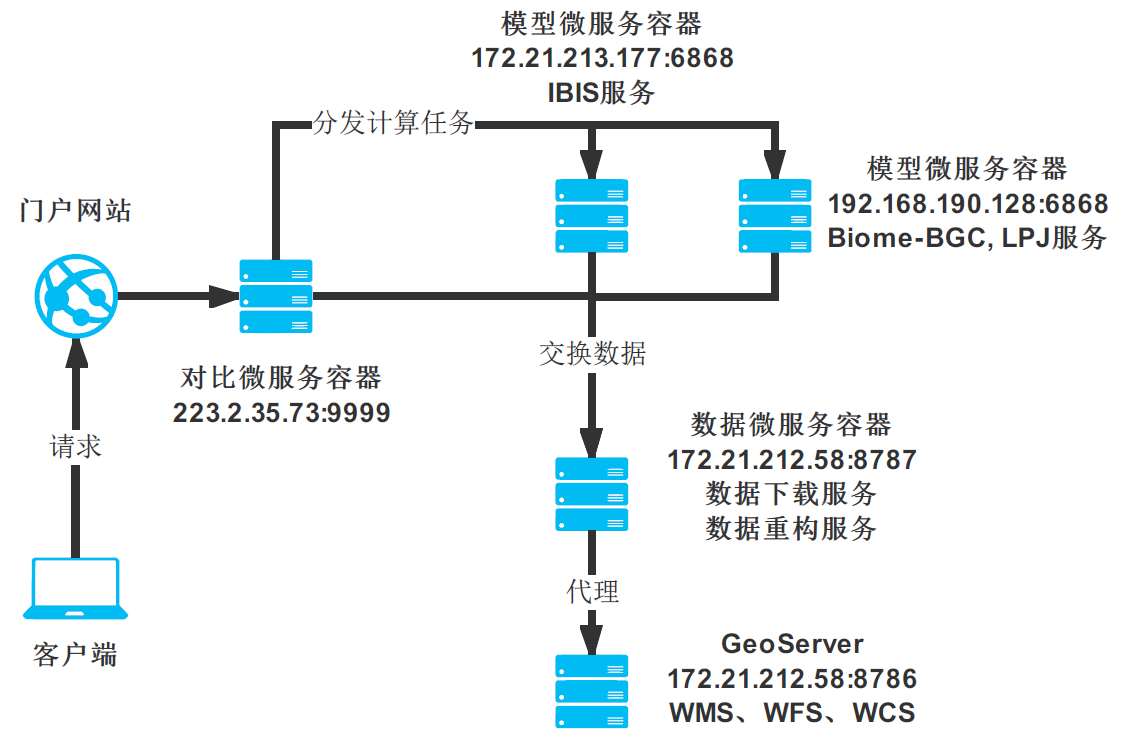
\includegraphics[width=1\textwidth]{server-topo}
    \caption{模型对比服务器网络拓扑图}
    \label{fig:server-topo}
\end{figure}

\subsection{微服务容器}
服务容器作为服务的承载工具,它本身并不处理非常复杂的计算逻辑,而是将CPU密集型操作交给它所容纳的服务,所以服务容器是IO密集型的程序,他需要处理高并发的HTTP请求。Node.js作为异步编程的代表,天生适合这种场景,所以本文选择Node.js作为后台服务容器开发语言,使用MongoDB管理数据。由于Node.js的单线程特性,它本身并不稳定,所以使用PM2进行单台服务节点上Node.js应用的负载均衡。

\begin{figure}[!htbp]
    \centering
    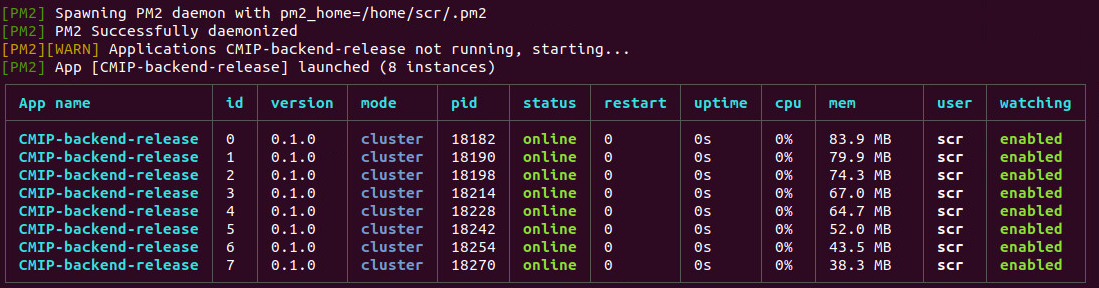
\includegraphics[width=1\textwidth]{PM2}
    \caption{PM2负载均衡管理}
    \label{fig:ms-LB}
\end{figure}

微服务容器作为面向管理员的后台管理工具,数据管理容器、模型计算容器和模型对比容器都具有很多通用的功能,如图~\ref{fig:service-container-common-fn}所示,微服务容器可以对服务进行管理,包括发布、注销、实例管理等,此外,还可以对服务器性能进行监控。

\begin{figure}[!htbp]
    \centering
    \subcaptionbox{服务列表、重新发布、注销\label{fig:service-publish-removal}}{
\includegraphics[width=.48\textwidth]{ms-step}}
    \hfill
    \subcaptionbox{服务上传部署发布\label{fig:service-deploy}}{
\includegraphics[width=.48\textwidth]{ms-step}} \\
    \subcaptionbox{服务实例管理\label{fig:insitance-manage}}{
\includegraphics[width=.48\textwidth]{ms-step}}
    \hfill
    \subcaptionbox{服务器性能监测\label{fig:monitor}}{
\includegraphics[width=.48\textwidth]{ms-step}}
    \caption{微服务容器通用功能}
    \label{fig:service-container-common-fn}
\end{figure}

除了通用功能,数据管理容器通过Nginx的消息中转还支持使用GeoServer发布WMS、WFS、WCS服务(图~\ref{fig:geoserver}),模型对比容器支持对计算节点进行管理(图~\ref{fig:api-gateway-children})。

\begin{figure}[!htbp]
    \centering
    
\includegraphics[width=1\textwidth]{ms-step}
    \caption{GeoServer发布数据服务}
    \label{fig:geoserver}
\end{figure}

\begin{figure}[!htbp]
    \centering
    
\includegraphics[width=1\textwidth]{ms-step}
    \caption{API网关(对比服务容器)上注册的子节点}
    \label{fig:api-gateway-children}
\end{figure}

\subsection{陆地生态系统碳循环模型对比门户网站}
面向开放式模型计算和对比的需求,本文构建了一个门户网站,作为共享对比方案和对比结果的入口。一方面可以将对比过程和结果公开化,降低碳循环模型的使用难度,另一方面可以激励模式组的模型通过封装加入进来,促进碳循环研究的发展。门户网站的主要功能模块设计为如图\ref{fig:system-module},功能模块分为资源模块、对比业务模块、结果展示模块和用户管理模块,其中资源模块包括模型资源和数据资源;对比业务模块则对应于对比话题、对比方案和对比任务;结果展示模块基于所有对比任务的执行结果,将对比结果展示出去;用户模块包括用户的个人资源管理。门户网站的登录、注册和首页如图~\ref{fig:portal-index}所示。

\begin{figure}[!htbp]
    \centering
    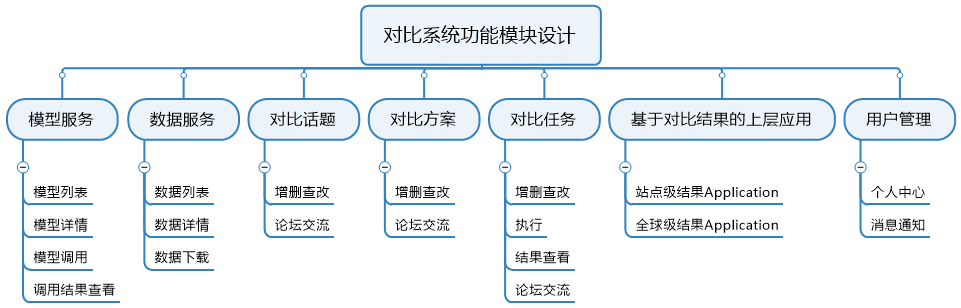
\includegraphics[width=1\textwidth]{system-module}
    \caption{对比系统功能模块设计}
    \label{fig:system-module}
\end{figure}

\begin{figure}[!htbp]
    \centering
    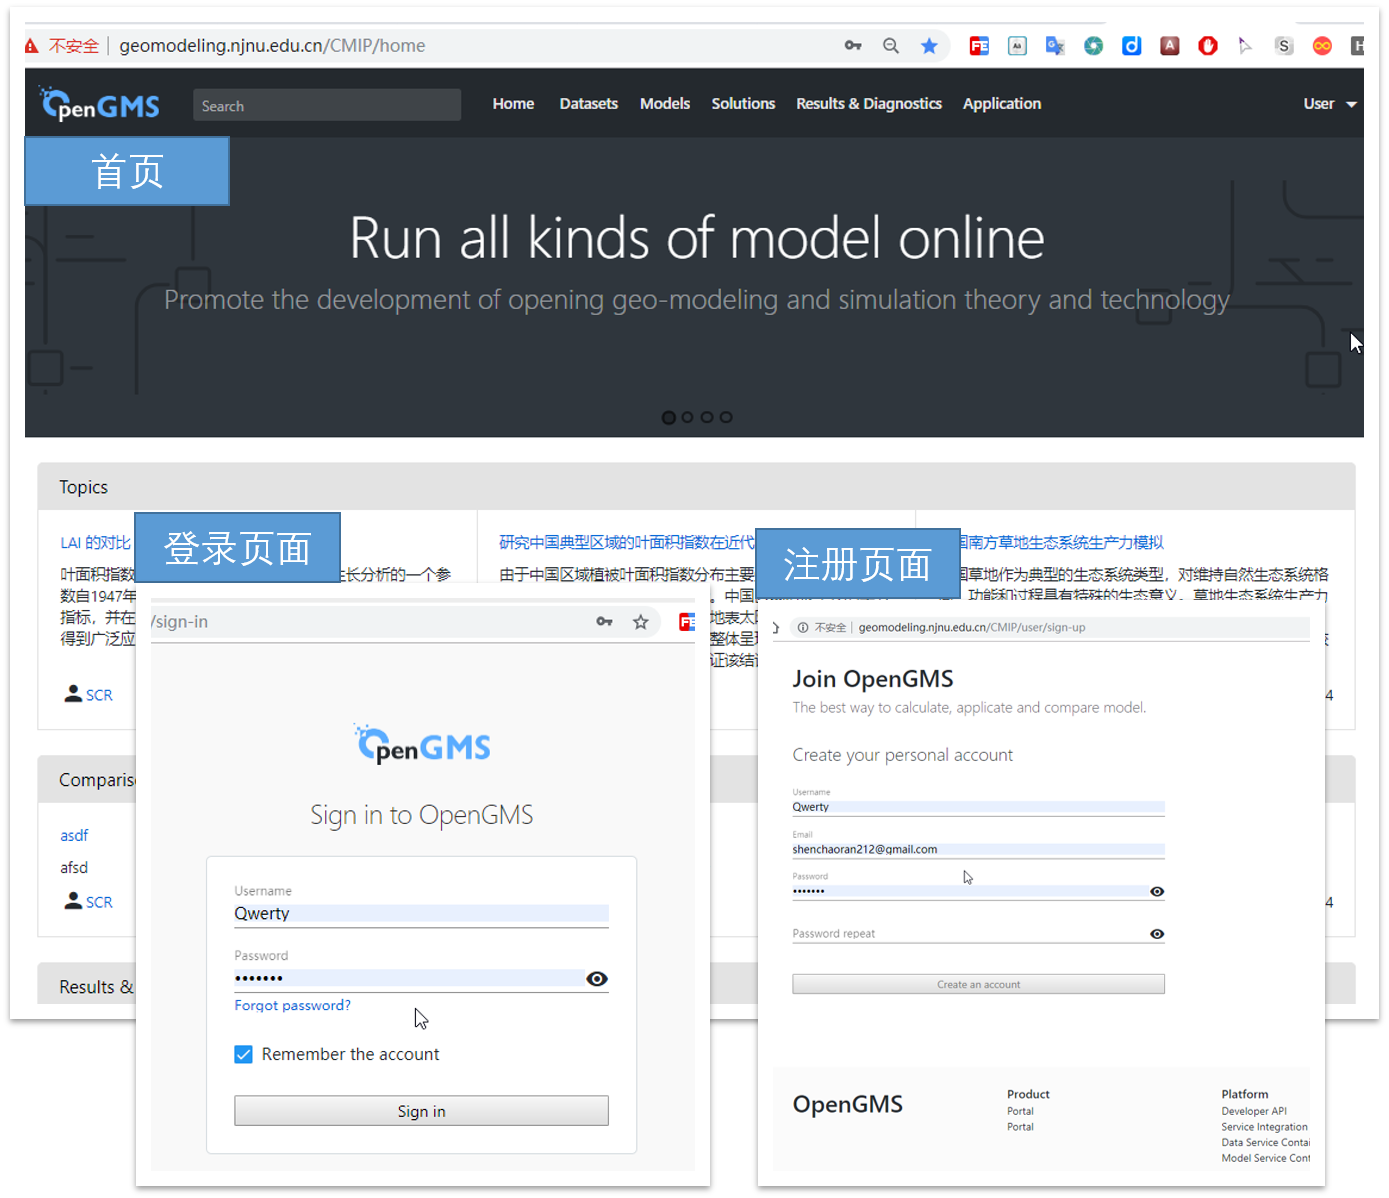
\includegraphics[width=.7\textwidth]{portal-index}
    \caption{门户网站首页和注册登录页面}
    \label{fig:portal-index}
\end{figure}

\begin{figure}[!htbp]
    \centering
    \subcaptionbox{模型资源和数据资源列表\label{fig:ms-data-resource}}{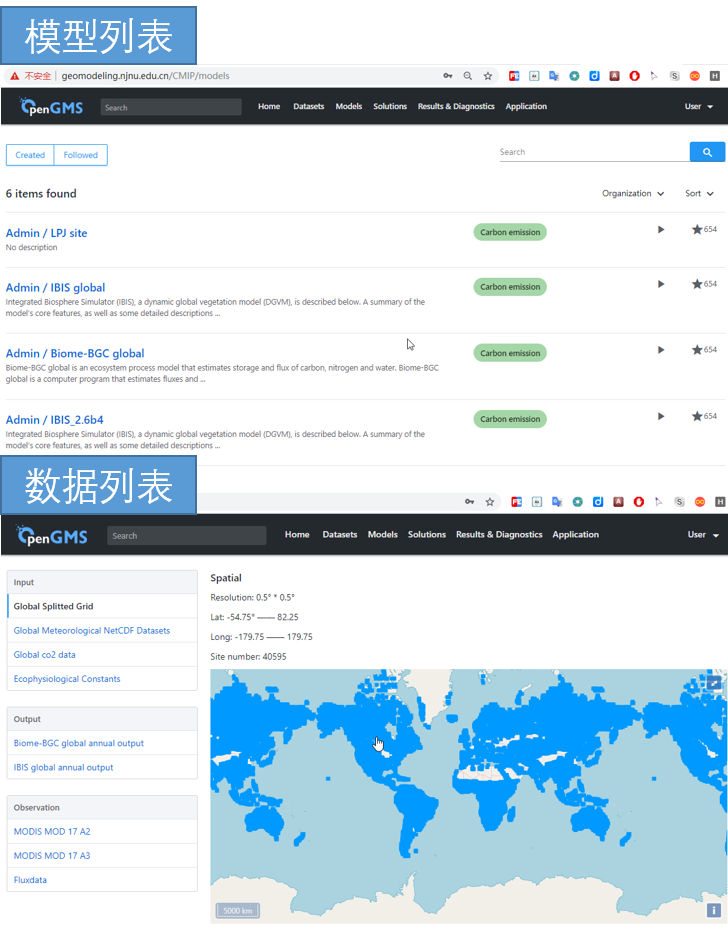
\includegraphics[width=.5\textwidth]{ms-data-resource}}
    \hfill
    \subcaptionbox{模型服务调用\label{fig:ms-invoke}}{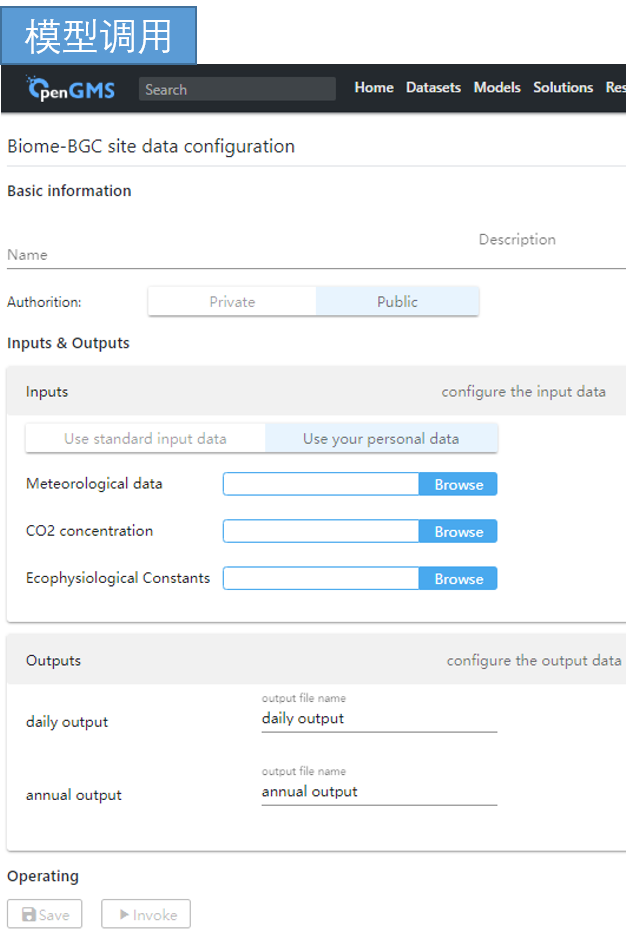
\includegraphics[width=.43\textwidth]{ms-invoke}}
    \caption{门户网站模型和数据资源}
    \label{fig:portal-resource}
\end{figure}

\begin{figure}[!htbp]
    \centering
    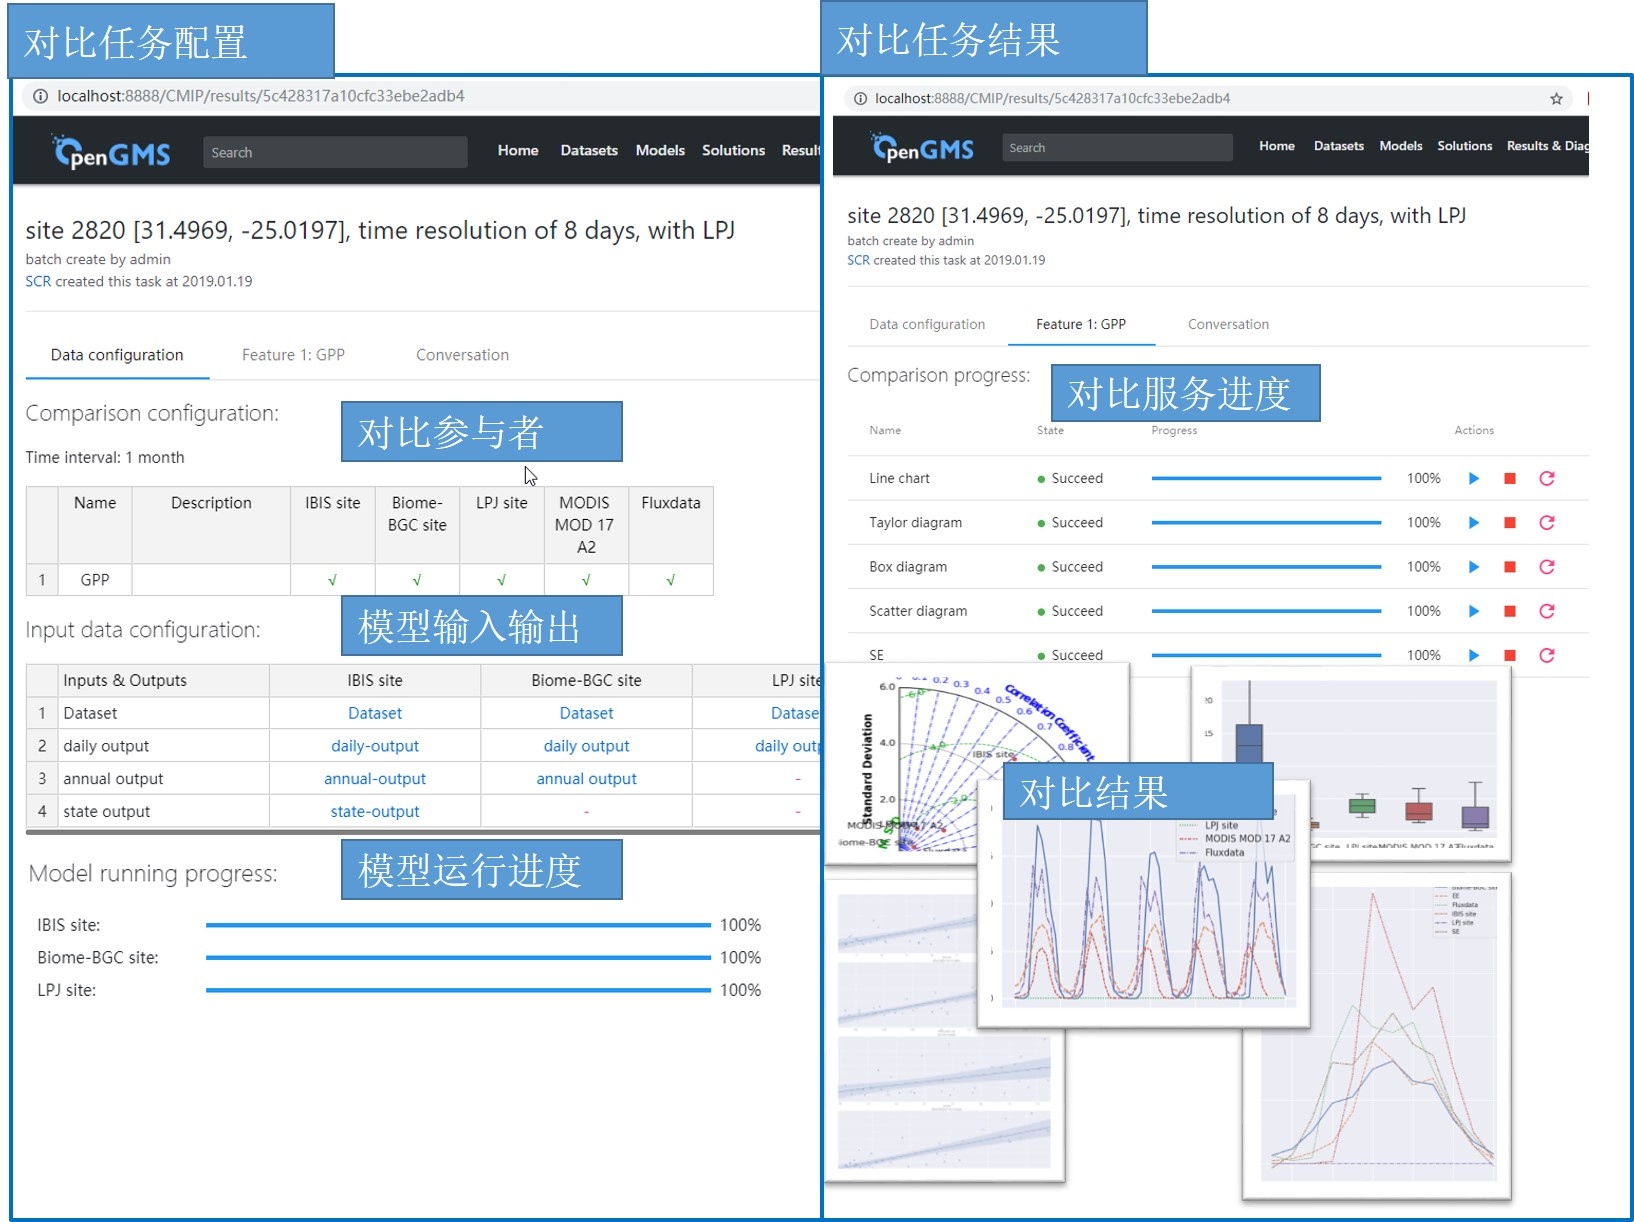
\includegraphics[width=1\textwidth]{task-cfg-result}
    \caption{对比任务配项和结果}
    \label{fig:task-cfg-result}
\end{figure}

\begin{figure}[!htbp]
    \centering
    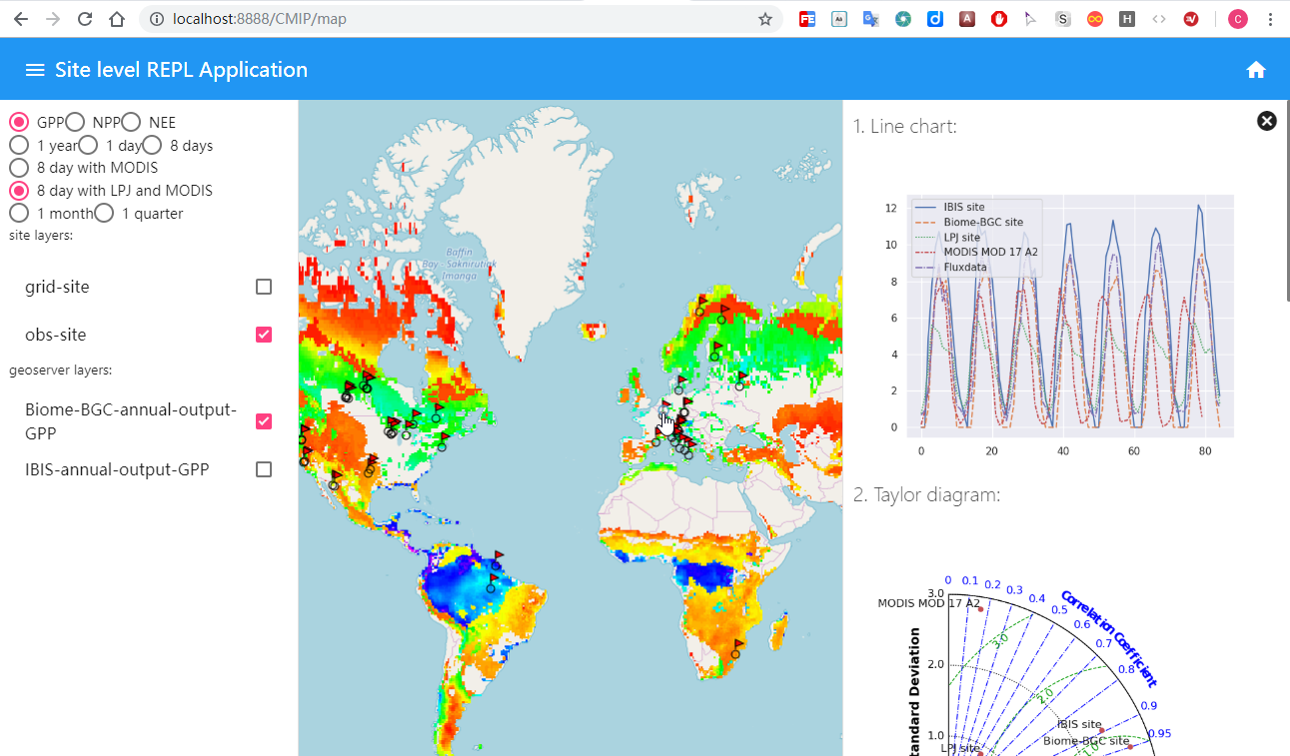
\includegraphics[width=.8\textwidth]{site-REPL}
    \caption{站点级对比结果查询应用}
    \label{fig:site-REPL}
\end{figure}

\section{实验案例}
\label{sec:experiments}
% GPP是评估。。,本文以同样的气象数据、和土壤数据驱动IBIS、Biome-BGC和LPJ,并参考MODIS GPP陆面产品,从单站点、多站点和全球三个维度分别对比四个模型的差异。
\subsection{单站点对比}
单站点层次上的对比方案通过第~\ref{sec:cmp-CSDL}节阐述的对比方案描述语言表达、执行、存储,实现了在站点层次上的共享和重用,对比方案配置观测站点的数据后形成对比任务。以AT-Neu站点为例,其基本信息如表~\ref{tab:site-AT-Neu}所示,统计对比结果如表~\ref{tab:site-AT-Neu-stat}所示,可视化对比结果如图~\ref{fig:visual-cmp-rst}所示。结果表明,三个模型模拟的结果较为一致,IBIS模拟结果偏高,Biome-BGC在均值、标准差、均方根误差、相关系数和效率系数等方面都与观测数据更为一致。

\noindent\begin{table}[!htbp]
    \begin{minipage}[t]{.3\textwidth}
        \centering
        \caption{AT-Neu站点信息}
        \label{tab:site-AT-Neu}
        \begin{tabular}{ll}
            \Xhline{1.5pt}
            站点名 & AT-Neu \\
            经度 & 11.3175 \\
            纬度 & 47.1167 \\
            高程 & 970m \\
            植被类型 & 草地 \\
            数据范围 & 2002-2012 \\
            \Xhline{1.5pt}
        \end{tabular}
    \end{minipage} %
    \begin{minipage}[t]{.62\textwidth}
        \centering
        \caption{AT-Neu站点的统计对比结果}
        \label{tab:site-AT-Neu-stat}
        \begin{tabular}{lrrrrr}
            \Xhline{1.5pt}
            & IBIS & Biome-BGC & LPJ & MODIS & Fluxnet \\
            \Xhline{1.5pt}
            MEAN & 7.96 & 4.22 & 2.61 & 2.07 & 5.56 \\
            STD & 6.91 & 2.63 & 2.52 & 2.12 & 4.73 \\
            RMSE & 5.32 & 3.17 & 4.14 & 5.41 & 0 \\
            COEF & 0.70 & 0.82 & 0.83 & 0.48 & 1 \\
            NSE & -0.2 & 0.55 & 0.23 & -0.31 & 0 \\
            \Xhline{1.5pt}
        \end{tabular}
    \end{minipage}
\end{table}

\begin{figure}[!htbp]
    \centering
    \subcaptionbox{时间序列折线图}{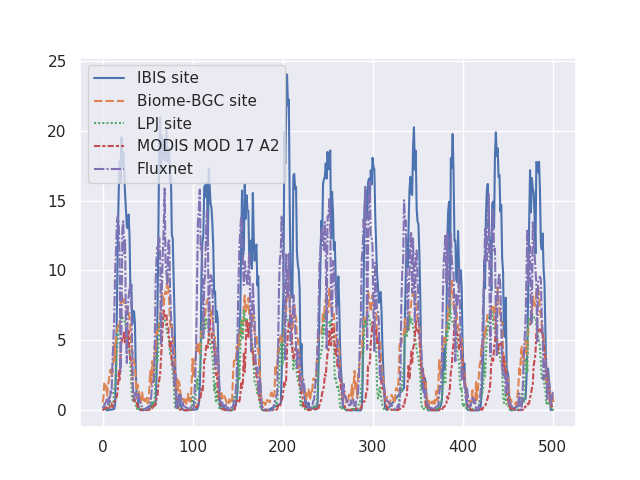
\includegraphics[width=0.49\textwidth]{22641-GPP-Line-chart}}
    \hfill
    \subcaptionbox{箱图}{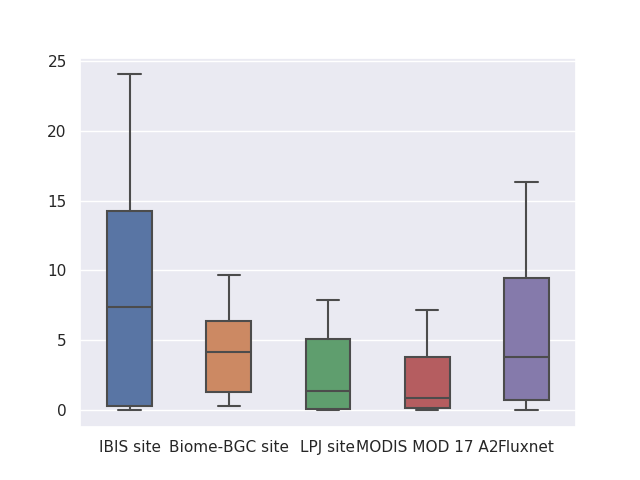
\includegraphics[width=0.49\textwidth]{22641-GPP-Box-diagram}} \\
    \subcaptionbox{泰勒图}{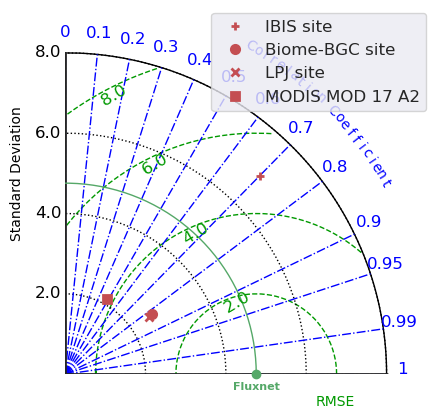
\includegraphics[width=0.6\textwidth]{22641-GPP-Taylor-diagram}}\\
    \caption{可视化对比结果}
    \label{fig:visual-cmp-rst}
\end{figure}

\subsection{基于植被功能类型的多站点差异性对比}
% 草地、灌木、落叶林、常绿林、混交林
由于每个站点的观测数据时间范围不同,在不同站点上不能选取相同的时间范围,本研究取模拟时间范围(1982-2013年)和观测站点的最长公共时间区间,将每个站点的模拟结果与观测数据进行对比,最后按照植被功能类型进行统计,得到不同植被功能类型下不同模型模拟的GPP和观测的GPP的平均值差异及相关系数表,如图~\ref{fig:heatmap-GPP-coef}所示,在CSH、ENF、MF三种植被类型中,四个模型模拟的相关系数都在0.6以上,而对EBF的模拟效果最差,相关性在0.21以下,同时,如图~\ref{fig:heatmap-GPP-mean}所示,IBIS模拟的GPP整体偏高2倍左右,总体来看,Biome-BGC和LPJ的模拟结果比MODIS在各种植被功能类型上都更要准确,其中,Biome-BGC无论是从相关性还是从均值分布上模拟能力都是最好的。
按照表~\ref{tab:site-PFT-stat}所统计的8中站点植被功能类型,将129个站点的分类统计。

\begin{figure}[!htbp]
    \centering
    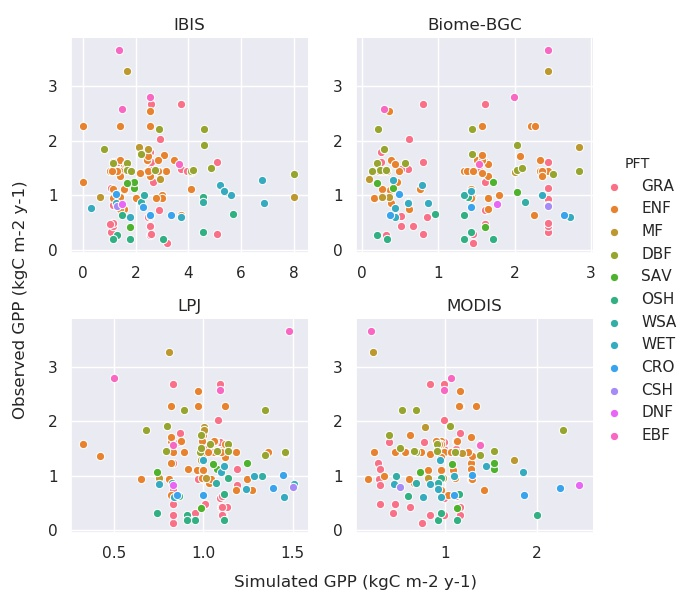
\includegraphics[width=1\textwidth]{scatter-GPP}
    \caption{129个站点GPP模拟值和观测值分布}
    \label{fig:api-gateway-children}
\end{figure}

\begin{figure}[!htbp]
    \centering
    \subcaptionbox{MEAN\label{fig:bar-GPP-mean}}{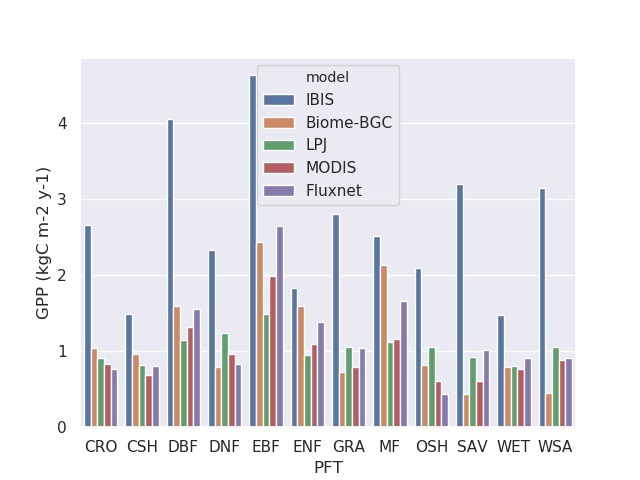
\includegraphics[width=.495\textwidth]{bar-GPP-mean}}
    \hfill
    \subcaptionbox{STD\label{fig:taylor-GPP-CSH}}{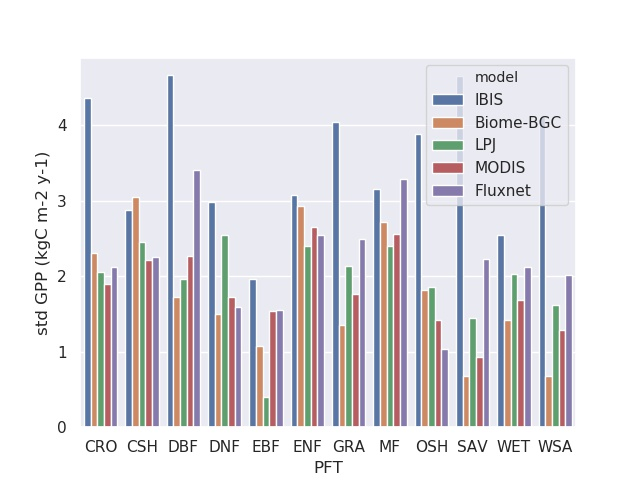
\includegraphics[width=.495\textwidth]{bar-GPP-std}} \\
    \subcaptionbox{COEF\label{fig:bar-GPP-mean}}{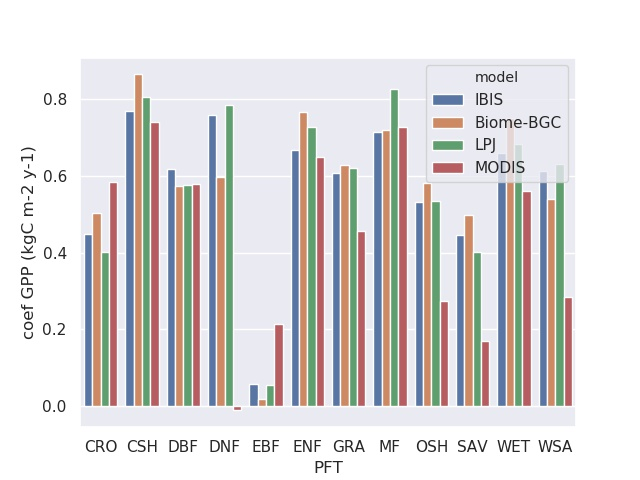
\includegraphics[width=.495\textwidth]{bar-GPP-coef}}
    \hfill
    \subcaptionbox{RMSE\label{fig:taylor-GPP-CSH}}{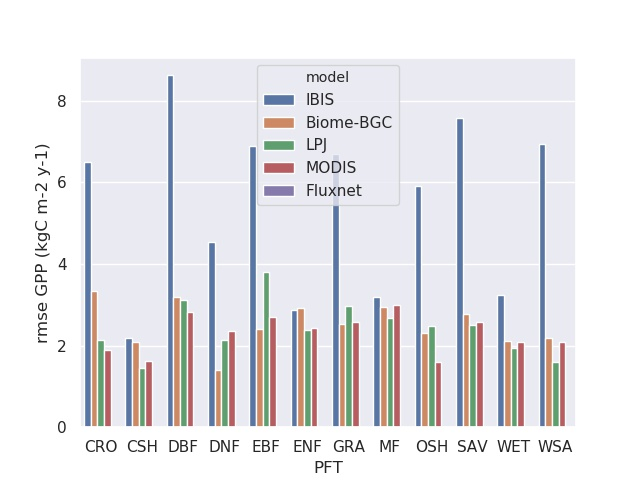
\includegraphics[width=.495\textwidth]{bar-GPP-rmse}} \\
    \caption{IBIS、Biome-BGC、LPJ和MODIS计算的GPP不同植被功能类型的统计指标柱状图}
    \label{fig:GPP-cmp-taylor}
\end{figure}

\begin{figure}[!htbp]
    \centering
    \subcaptionbox{OSH\label{fig:taylor-GPP-OSH}}{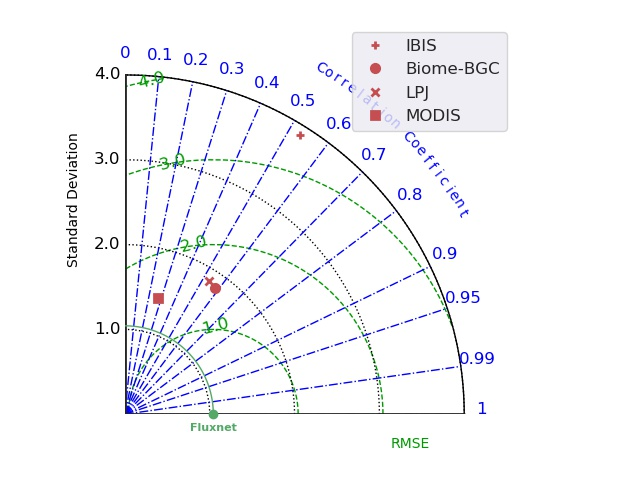
\includegraphics[width=.48\textwidth]{taylor-GPP-OSH}}
    \hfill
    \subcaptionbox{CSH\label{fig:taylor-GPP-CSH}}{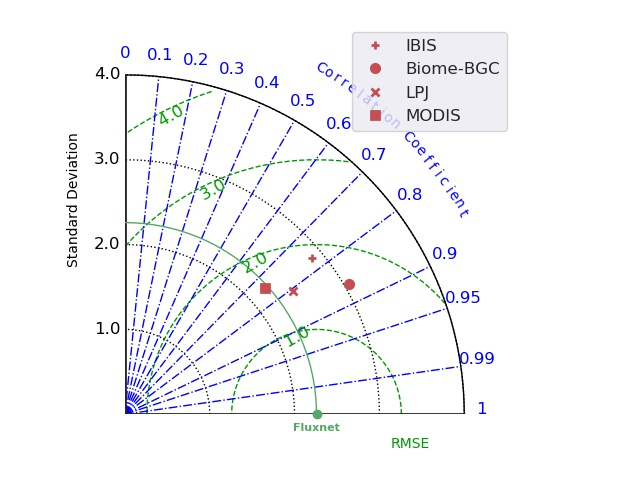
\includegraphics[width=.48\textwidth]{taylor-GPP-CSH}} \\
    \subcaptionbox{DBF\label{fig:taylor-GPP-DBF}}{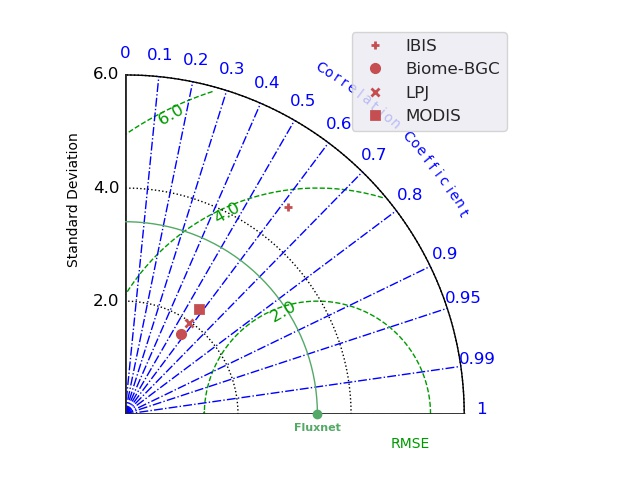
\includegraphics[width=.48\textwidth]{taylor-GPP-DBF}}
    \hfill
    \subcaptionbox{EBF\label{fig:taylor-GPP-EBF}}{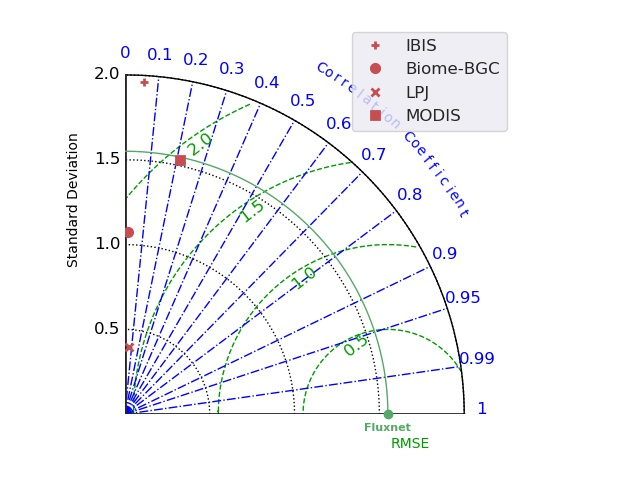
\includegraphics[width=.48\textwidth]{taylor-GPP-EBF}} \\
    \subcaptionbox{DNF\label{fig:taylor-GPP-DNF}}{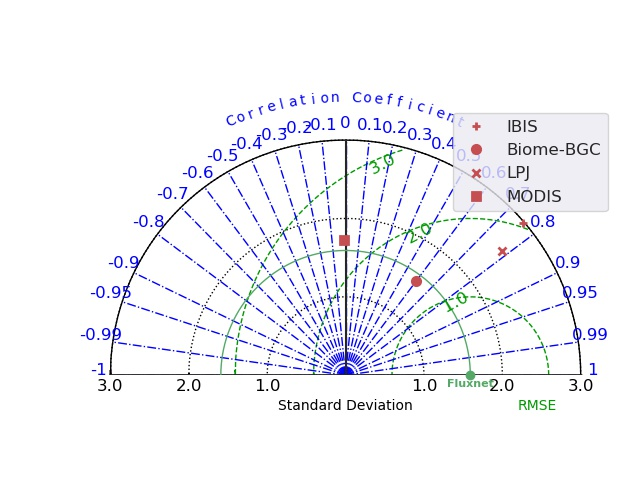
\includegraphics[width=.48\textwidth]{taylor-GPP-DNF}} 
    \hfill
    \subcaptionbox{ENF\label{fig:taylor-GPP-ENF}}{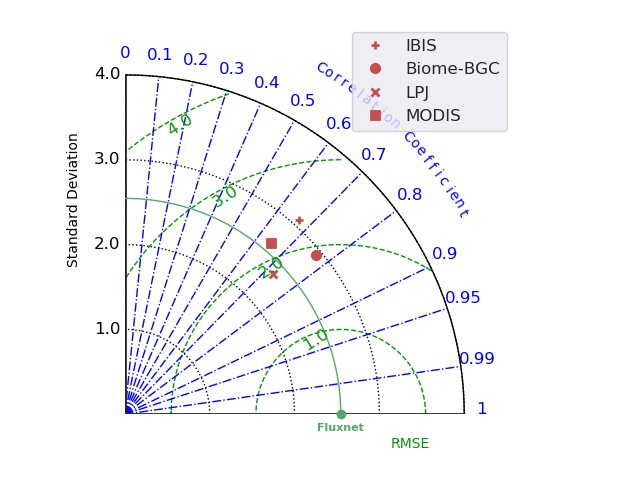
\includegraphics[width=.48\textwidth]{taylor-GPP-ENF}} \\
    \subcaptionbox{GRA\label{fig:taylor-GPP-GRA}}{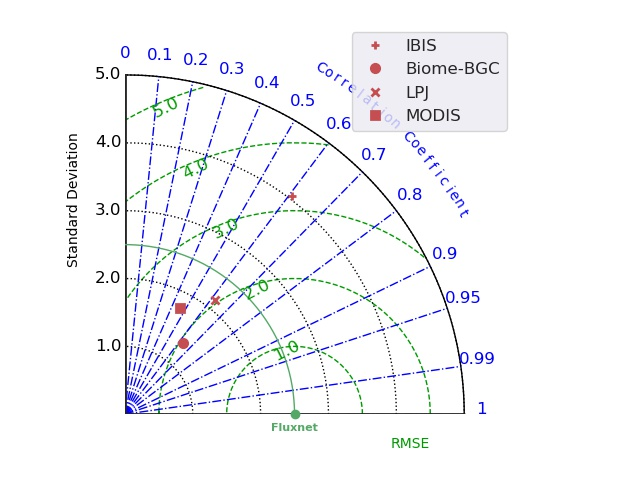
\includegraphics[width=.48\textwidth]{taylor-GPP-GRA}}
    \hfill
    \subcaptionbox{SAV\label{fig:taylor-GPP-SAV}}{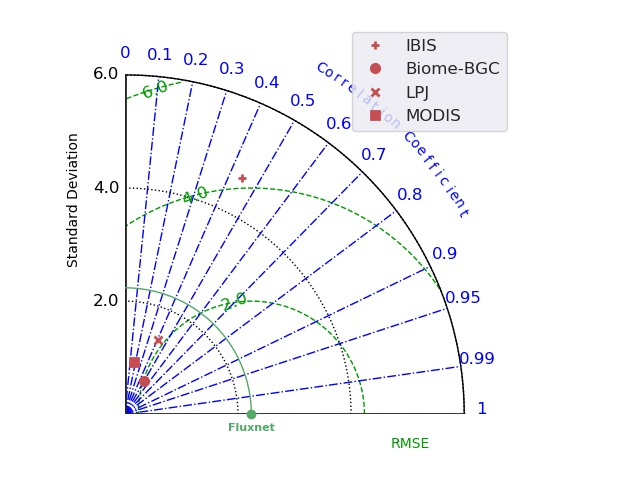
\includegraphics[width=.48\textwidth]{taylor-GPP-SAV}}
    % \hfill
    % \subcaptionbox{WSA\label{fig:taylor-GPP-WSA}}{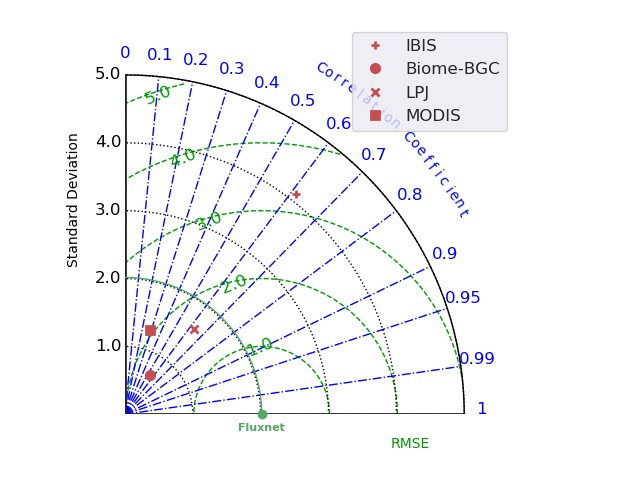
\includegraphics[width=.48\textwidth]{taylor-GPP-WSA}} 
    % \hfill
    % \subcaptionbox{CRO\label{fig:taylor-GPP-CRO}}{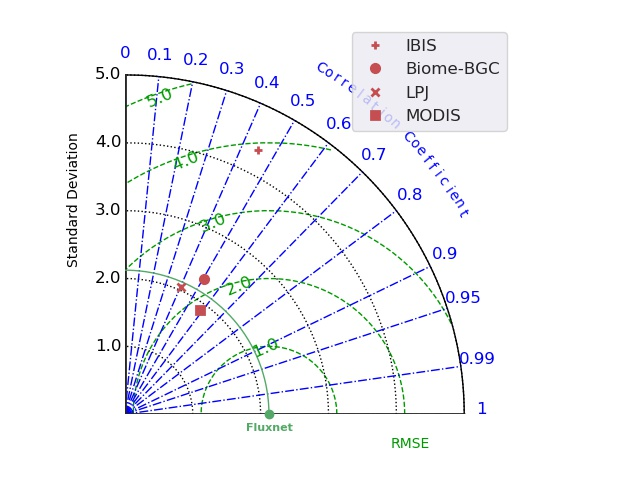
\includegraphics[width=.48\textwidth]{taylor-GPP-CRO}}
    % \subcaptionbox{MF\label{fig:taylor-GPP-MF}}{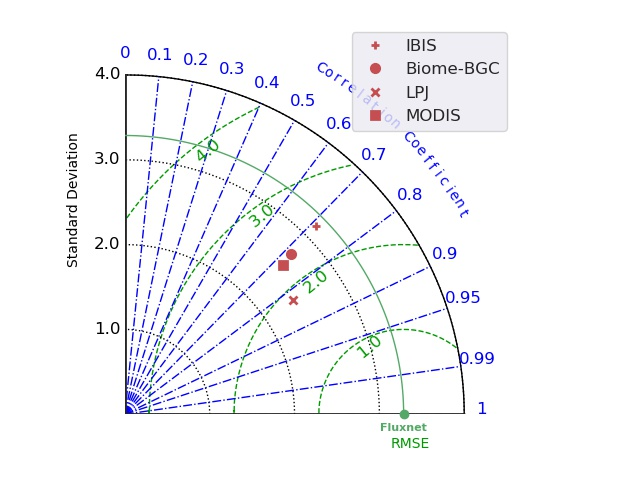
\includegraphics[width=.48\textwidth]{taylor-GPP-MF}} \\
    % \subcaptionbox{WET\label{fig:taylor-GPP-WET}}{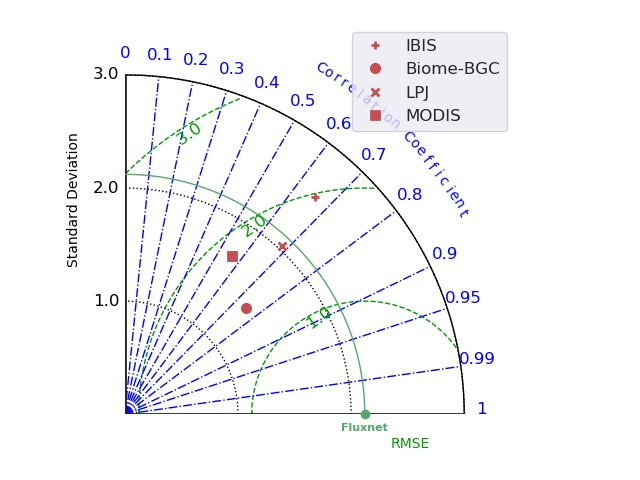
\includegraphics[width=.48\textwidth]{taylor-GPP-WET}}
    \caption{IBIS、Biome-BGC、LPJ和MODIS计算的GPP不同植被功能类型的雷达图}
    \label{fig:GPP-cmp-taylor}
\end{figure}


\subsection{基于全球网格点的时空分布格局对比}
\subsubsection{时间变化对比}
本文基于全球范围内划分的网格点的模拟结果,以MOD17A2的模拟结果进行交叉对比,如图~\ref{fig:GPP-annual}三个模型模拟的GPP都承缓慢上升趋势,其中Biome-BGC的结果和MODIS的模拟结果最为接近,而IBIS整体偏高,LPJ整体偏低。4个模型模拟的GPP季节分布规律如图~\ref{fig:GPP-monthly},不论南北半球都是夏季GPP升高,冬季GPP降低。

\begin{figure}[!htbp]
    \centering
    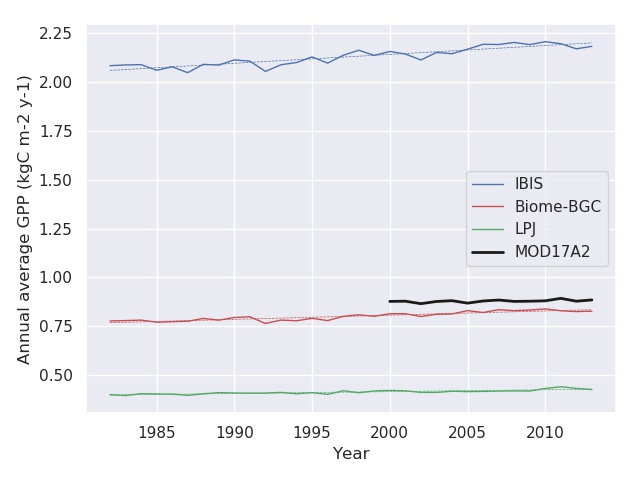
\includegraphics[width=.8\textwidth]{GPP-annual}
    \caption{IBIS、Biome-BGC、LPJ和MODIS模拟的GPP的年际变化趋势}
    \label{fig:GPP-annual}
\end{figure}

\begin{figure}[!htbp]
    \centering
    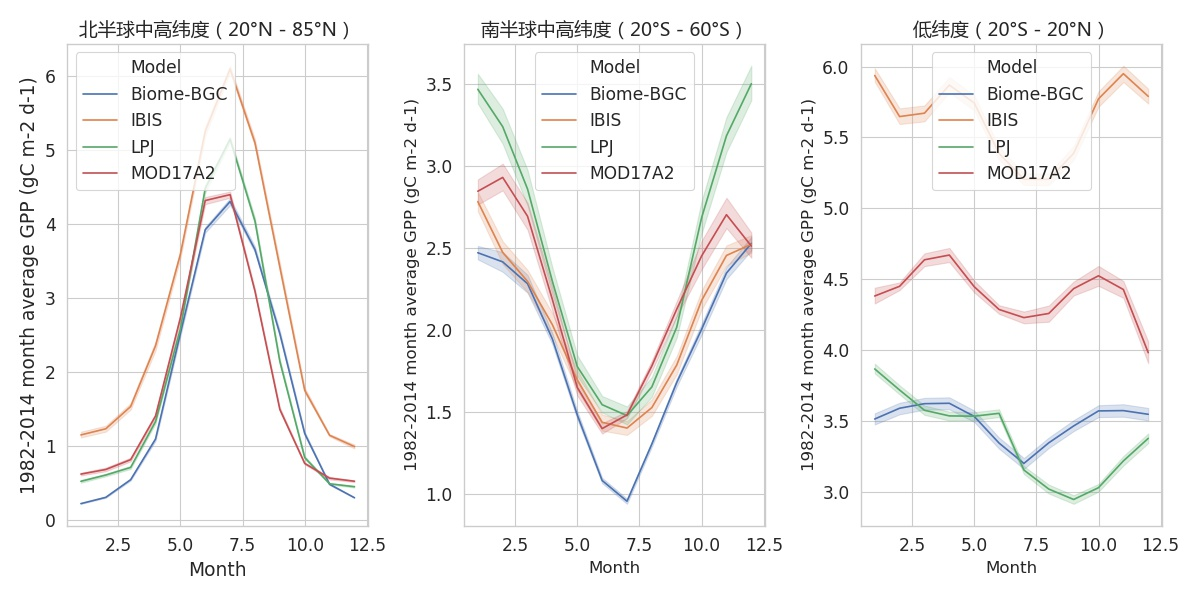
\includegraphics[width=1\textwidth]{GPP-monthly}
    \caption{IBIS、Biome-BGC、LPJ和MODIS模拟的GPP的季节变化规律}
    \label{fig:GPP-monthly}
\end{figure}


\subsubsection{空间格局对比}
% TODO 全球总GPP
从空间格局上来看,Biome-BGC模拟结果与MOD17A2的结果最为接近,而IBIS全球范围内都偏高,而LPJ模拟的整体稍微偏低。从纬度的分布上来看,如图~\ref{fig:GPP-lat},GPP的分布存在着明显的维度规律,在低纬度GPP最高,在高纬度GPP偏低,GPP在$0^{\circ}$、北纬$20^{\circ}$、南纬$35^{\circ}$存在三个峰值。三个模型中Biome-BGC与MODIS的结果最为一致,而在低纬度与MODIS模拟差异较大。

\begin{figure}[!htbp]
    \centering
    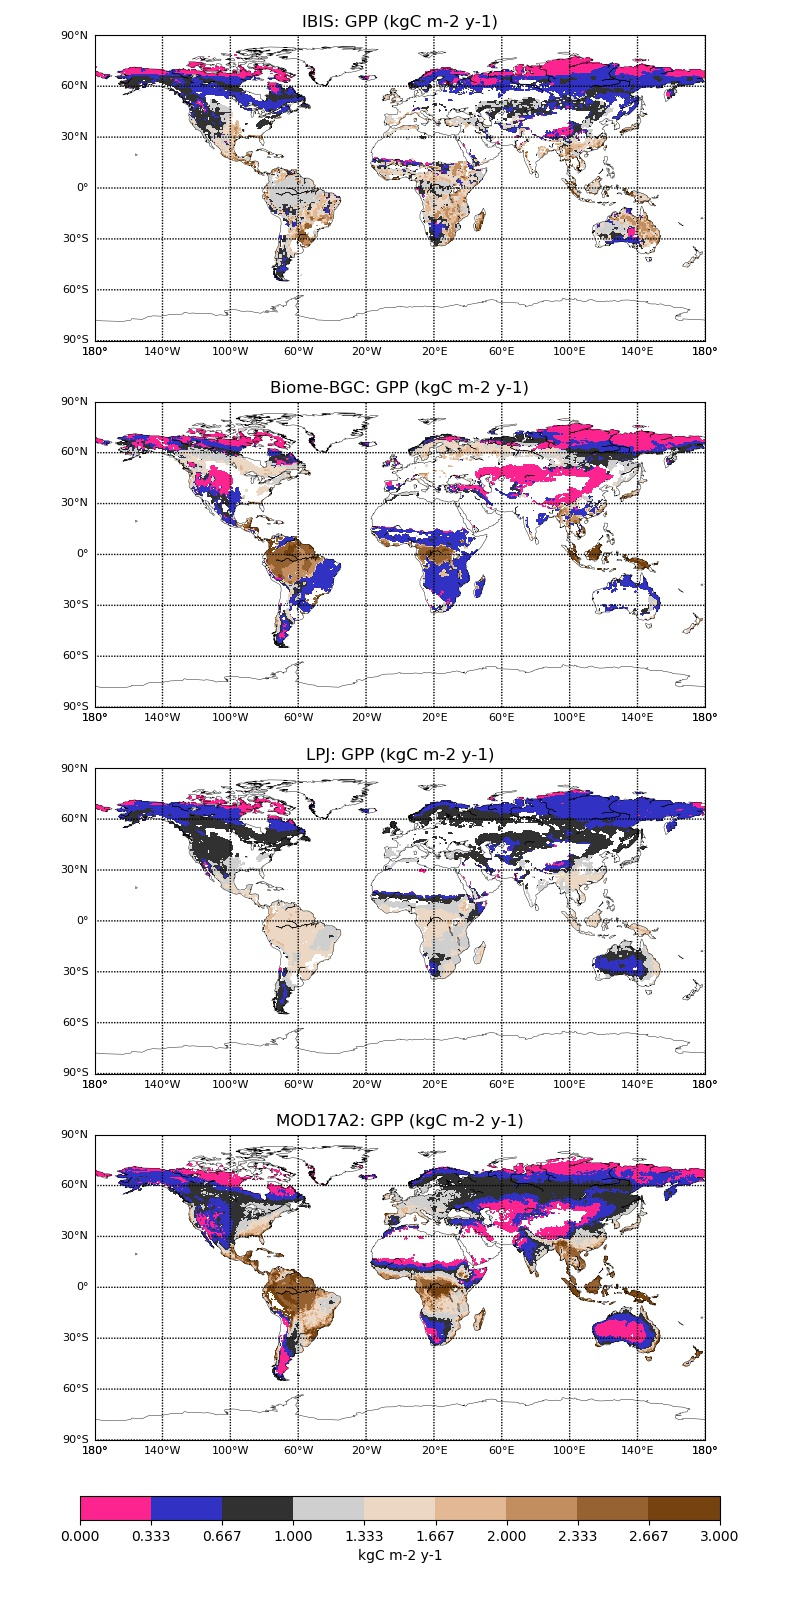
\includegraphics[width=1\textwidth]{GPP.pdf}
    \caption{IBIS、Biome-BGC、LPJ和MODIS的GPP的空间分布格局对比}
    \label{fig:GPP}
\end{figure}

\begin{figure}[!htbp]
    \centering
    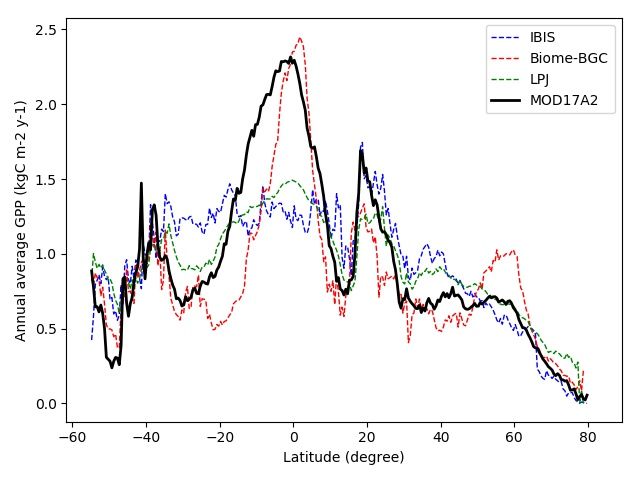
\includegraphics[width=1\textwidth]{GPP-lat}
    \caption{IBIS、Biome-BGC、LPJ和MODIS的GPP的纬向变化规律}
    \label{fig:GPP-lat}
\end{figure}